\documentclass[oneside,final,14pt,a4paper]{extreport}

\usepackage{tempora} % Times New Roman alike font  

\usepackage{vmargin}
\setpapersize{A4}
\setmarginsrb{2.5cm}{2.2cm}{2.2cm}{2.2cm}{0pt}{10mm}{0pt}{13mm}
\usepackage{setspace}
\setstretch{1.5}
\usepackage{indentfirst}
\parindent=1.25cm

%%%%% ADDED TO SUPPORT TT BOLD FACES %%%%
\DeclareFontShape{OT1}{cmtt}{bx}{n}{<5><6><7><8><9><10><10.95><12><14.4><17.28><20.74><24.88>cmttb10}{}
\renewcommand{\ttdefault}{pcr}
%%%%% END %%%%%%%%%%%%%%%%%%%%%%%%%%%%%%% 

\usepackage{atbegshi,picture}
\usepackage[T1,T2A]{fontenc}
\usepackage[utf8]{inputenc}

\usepackage[english]{babel}
\usepackage[backend=biber,style=ieee,autocite=inline,maxnames=3,mincitenames=1,maxcitenames=1]{biblatex}
\bibliography{ref.bib}
\DefineBibliographyStrings{english}{%
  bibliography = {References},}
\usepackage{blindtext}

\usepackage{pdfpages}
\newenvironment{bottompar}{\par\vspace*{\fill}}{\clearpage}
\usepackage{amsmath,amsfonts}
\usepackage{url}
\usepackage{amsthm}
\newtheorem{theorem}{Theorem}
\newtheorem{corollary}{Corollary}
\newtheorem{lemma}{Lemma}
\newtheorem{proposition}{Proposition}
\theoremstyle{definition}
\newtheorem{definition}{Definition}
\theoremstyle{remark}
\newtheorem*{remark}{Remark}
\theoremstyle{remark}
\newtheorem*{example}{Example}

\usepackage{float}
\usepackage{graphicx}
\graphicspath{{figs/}} %path to images
\usepackage{array}
\usepackage{multirow,array}
\usepackage{caption}
\usepackage{subcaption}
\usepackage{hyperref}
\hypersetup{colorlinks=true, linkcolor=black, citecolor=black}
\urlstyle{same}

\usepackage{paralist}
\usepackage{listings}
\usepackage{zed-csp}
\usepackage{fancyhdr}
\usepackage{csquotes}
\usepackage{color}
% \usepackage{anyfontsize}
% \usepackage{mathptmx}
% \usepackage{t1enc}

\usepackage{chngcntr}
\usepackage{upgreek} 
\usepackage{bm}
\usepackage{hyperref}
\usepackage{booktabs}
\usepackage{multirow}
\usepackage{longtable}
\usepackage[font=singlespacing, labelfont=bf]{caption}
%Hints
\newcommand\pic[1]{(Fig. \ref{#1})} %Ref on figure
\newcommand\tab[1]{(Tab. \ref{#1})} %Ref on table

\setlength{\headheight}{32.0976pt}
\usepackage{enumitem}
\newlist{inlinelist}{enumerate*}{1}
\setlist*[inlinelist,1]{%
  label=(\arabic*),
}

% \setcounter{secnumdepth}{4}
\captionsetup[table]{labelfont={normalfont}, name={TABLE}, labelsep={newline}}
\setlength{\parindent}{2em} 
\DeclareCaptionLabelSeparator{figSep}{.\quad}
\captionsetup[figure]{labelfont={normalfont}, name={Fig.}, labelsep=period}
\counterwithin{figure}{chapter}

% \usepackage{titlesec}
% \titleformat{\section}[hang]{\fontsize{20}{24}\selectfont\filcenter}{\Roman{section}}{1em}{}
% \titleformat{\subsection}[hang]{\itshape}{\Alph{subsection}.}{1em}{}[]
% \titleformat{\subsubsection}[runin]{\itshape}{\arabic{subsubsection})}{1em}{}[$:$]
% \titlespacing{\subsubsection}{1em}{1em}{1em}
% \titleformat{\paragraph}[runin]{\itshape}{\alph{paragraph})}{1em}{}[$:$\quad]
% \titlespacing{\paragraph}{2em}{1em}{1em}

\usepackage{placeins} % for \FloatBarrier

\pagestyle{fancyplain}

% remember section title
\renewcommand{\chaptermark}[1]%
	{\markright{\chaptername~\thechapter~--~#1}}

% subsection number and title
\renewcommand{\sectionmark}[1]%
	{\markright{\thesection\ #1}}

\rhead[\fancyplain{}{\bf\leftmark}]%
      {\fancyplain{}{\bf\thepage}}
\lhead[\fancyplain{}{\bf\thepage}]%
      {\fancyplain{}{\bf\rightmark}}
\cfoot{} %bfseries


\newcommand{\dedication}[1]
   {\thispagestyle{empty}
     
   \begin{flushleft}\raggedleft #1\end{flushleft}
}

\begin{document}
\renewcommand{\figureautorefname}{Fig.}
\renewcommand{\chapterautorefname}{Chapter}
\renewcommand{\sectionautorefname}{Section}

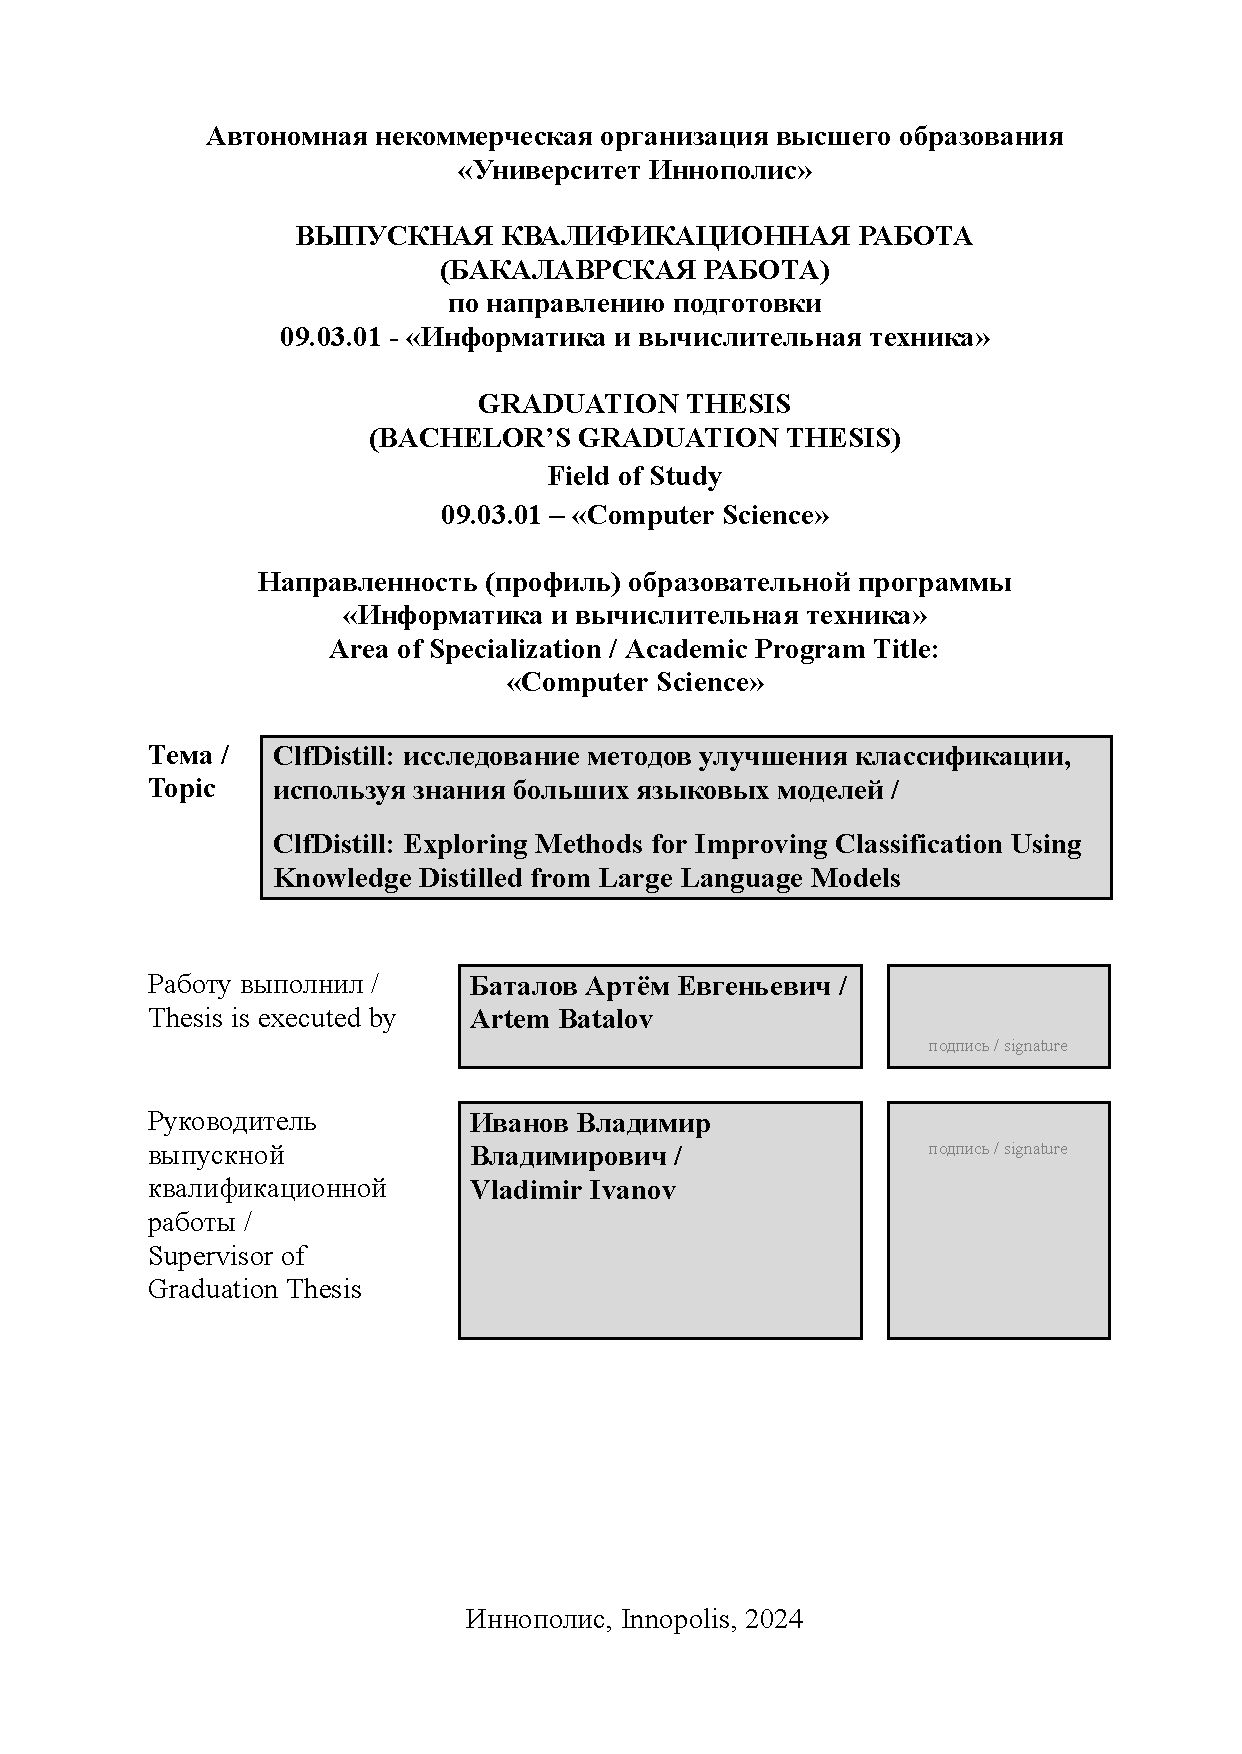
\includepdf[pages=-,offset=25.5mm -25.5mm]{title.pdf}
\tableofcontents
\listoftables
\listoffigures
\newpage


\begin{abstract}
    % skip one line to make the abstract start with indent

    The exponential growth of transformer-based large language models (LLM) improved the state-of-the-art natural language processing field, offering unprecedented capabilities in performing complex language understanding tasks. However, the deployment of these models in real-world applications is hampered by their substantial computational and memory requirements. 
    
    To address this challenge, this thesis delves into the process of distilling an LLM into a sequence classification model. The aim is to compress the vast knowledge of LLMs into smaller, more efficient models that are suitable for practical applications. The study is primarily focused on black-box methods, a unique approach where knowledge is transferred from the LLM to a smaller model based solely on the LLM's output, without access to its internal parameters.

    After a series of experiments, I propose a novel distillation pipeline that combines the generative capabilities of sequence-to-sequence models with the classification strengths of state-of-the-art encoder models. This pipeline effectively distills knowledge from the T5 model to the RoBERTa model, resulting in improved performance on the test set of the WOS dataset on 1-2\%.
\end{abstract}

\setcounter{page}{7}
% set manually the number, from which Chapter 1 starts!
% Why do we put 7 in this case?
% Title page - page 1
% Contents - page 2, page 3
% List of tables - page 4
% List of figures - page 5
% Abstract - page 6
% Chapter 1 - page 7
% In your thesis the counter number can be different, please count carefully and insert the corresponding number.

\chapter{Introduction}
\label{chap:intro}

The Transformer Architecture has improved the state-of-the-art in various sequence modeling tasks \cite{attention}. Transformer-based Large Language Models (LLM), such as GPT \cite{gpt}, with billions of parameters, have displayed near-human or sometimes even superhuman performance on specific tasks. The capability to process and generate coherent and contextually relevant text has led to their widespread adoption. However, Transformer's and LLM's high efficiency comes at the cost of a quadratic computational and memory complexity concerning the sequence length, so deploying such models in real-world scenarios can be financially and environmentally costly.

In the realm of research and development, expansive interest focuses on applying LLM in production environments, emphasizing computational efficiency. This thesis explores knowledge distillation (KD) methods and other techniques to reduce model size and complexity, making them more practical and sustainable for real-world applications.

In this study, I mainly consider the comparative analysis and application of KD techniques in the field of LLM\@. The primary objective of this research is to investigate the process of distilling an LLM into a text classification model and to evaluate the efficacy of this methodology in comparison with alternative approaches. The central thesis revolves around understanding how these KD methods can be leveraged to optimize LLMs, making them more viable for practical applications and minimizing the degradation of their capabilities.

In chemistry, distillation refers to separating the components of a liquid mixture consisting of two or more distinct substances. This separation process is achieved by selectively boiling the mixture and subsequently condensing the vapors in a distillation apparatus, commonly known as a still. This technique leverages differences in the boiling points of the substances to effect their separation, allowing each component to be isolated based on its specific boiling temperature \cite{chem_distil}.

Transitioning from the concept of chemical distillation to machine learning (ML) knowledge distillation, we observe a thematic shift from physical separation processes to the abstraction of knowledge transfer within computational models. In ML, particularly in the context of KD, the process is metaphorically similar but functionally distinct. KD involves transferring knowledge from a larger, more complex model to a smaller, more efficient one. The `boiling down' of knowledge occurs not through heat but through training processes where the student model learns to mimic the performance of the teacher model. This is achieved by optimizing the student model to reproduce the output distributions of the teacher model, effectively condensing the expansive knowledge of the teacher into a more compact form suitable for efficient deployment \cite{distilling}.

While both processes differ vastly in their mechanisms — physical versus computational — they share a core principle of extracting and isolating essential features from a broader set. In chemistry, this is the individual components of a mixture; in machine learning, it is the critical information and predictive capabilities contained within large datasets and complex model architectures.

KD techniques are mainly categorized into white-box and black-box approaches. \textbf{White-box KD} \cite{distilling}, where the internal parameters of the teacher model are accessible like LLaMA \cite{llama,llama2} and Mistral \cite{mistral}, is becoming more valuable for the research community and industry, as it enables student models to receive more comprehensive training signals from the teacher models, potentially leading to improved performance. Additionally, it is important to note that in the past six months, some open-source LLMs have been released that either match or surpass the performance of GPT-3.5 across various benchmarks. These emerging models are noteworthy for their competitive performance levels and the accessibility they offer to their parameters and hidden states, making them ideal candidates for white-box KD research. Notably, while white-box KD has been extensively applied to classification models and smaller language understanding models, its application to generative LLMs is not well-studied. Consequently, much additional work is required before a complete understanding can be reached. For more detailed information about white-box KD, including the latest research developments in this area, refer to \autoref{section:whitebox}.

On the other hand, \textbf{Black-box KD} (data-free knowledge distillation \cite{dfkd}, prompt-based distillation) involves using only the output predictions of teacher models. This method has shown effectiveness in refining smaller models by training them on response pairs generated by LLM API\footnote{application programming interface}, like GPT-3.5 and GPT-4.

The study focuses on black-box methods and includes a proposal for a novel distillation pipeline that combines the generative capabilities of sequence-to-sequence (Seq2Seq) models with the classification strengths of state-of-the-art encoder models.

The thesis is structured as follows. \autoref{chap:lr} presents some related work about knowledge distillation in ML models, highlighting recent advancements in the field of LLM\@. \autoref{chap:met} and \autoref{chap:impl} deal with the experimental setup, methodology of measuring the distillation effectiveness, experimental procedure description, and results. The respective analysis, discussions, and further work are presented in \autoref{chap:eval}. Finally, \autoref{chap:conclusion} presents conclusions of the entire work.


\chapter{Literature Review}
\label{chap:lr}

The structure of the literature review in this chapter is designed to offer an in-depth and complete insight into the concept of model distillation, particularly about the research question at hand. This review aims to elucidate the various facets of model distillation, including its theoretical foundations, practical applications, and relevance to the specific research question being addressed.

\section{Search Process}

Google Scholar was the primary digital platform for sourcing scholarly articles relevant to Knowledge Distillation techniques applied to LLMs. The search was conducted using a predefined set of keywords: \{Distillation, Large Language Model, Classification, Natural Language Processing\}. Furthermore, I scrutinized some references from the acquired articles to deepen my understanding of the subject matter. For a study to be included in this review, it needed to either detail a method of LLM distillation or provide sufficient background information to contextualize the research findings. I also set exclusion criteria; studies were disregarded if they lacked verifiable credibility, as indicated by insufficient citations, absence from prominent conferences, or non-publication in well-regarded scientific journals. Consequently, the majority of the selected studies were sourced from arXiv\footnote{\url{https://arxiv.org}}, where authors and institutes post electronic preprints and post-prints, which are moderated before but not peer-reviewed, and papers from the ACL and NeurIPS conferences, both of which are high-prestige venues with rigorous peer review processes.

\section{Knowledge distillation}

One of the paradigms for deriving a more compact model from a larger one or transferring the knowledge to another model is known as ``knowledge distillation.'' During this process, knowledge from a larger model (often called the teacher model) is transferred to a smaller model (student model). The fundamental premise behind this is that the teacher model has captured a deep understanding of the data, which can be imparted to a student model, ensuring that the smaller model performs at a level comparable to its bigger counterpart without consuming the same computational resources. This methodology initially became widespread for classification tasks within the realm of computer vision and has been effectively utilized across various fields, including LLMs.

\begin{figure}[hbt]
    \centering
    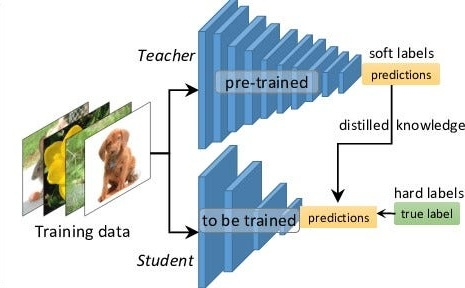
\includegraphics[width=0.7\linewidth]{figs/distillation.jpg}
    \caption{Distillation process. Source: \cite{kd_simplified}.}
    \label{fig:distillation}
\end{figure}

As shown in \autoref{fig:distillation}, the distillation typically trains the student the student model on a combination of the original dataset and the logits (soft outputs) produced by the teacher model. These outputs carry rich information about the data distribution, which aids the student model in capturing the nuances of complex decision boundaries. By leveraging the teacher model's expertise, the student model can learn more efficiently and produce results that are close to, and sometimes even surpass, the performance of the teacher model \cite{distilling}.

Kullback-Leibler (KL) Divergence loss \cite{kl} is a crucial aspect of the knowledge distillation training process. It quantifies the discrepancy between two probability distributions. Specifically, within the framework of model distillation, this loss assesses the divergence between the teacher and student model output distributions and allows you to train a student to minimize it.

The training loss is a linear combination (weighted sum) of the usual cross-entropy loss and KL divergence. The weight given to the distillation loss depends on the ratio of logits of the teacher and the student, making it adaptive and allowing the KL divergence component to have a more significant contribution when the teacher is more confident in the prediction than the student.

% As proposed by \citeauthor{multidistil} \cite{multidistil}, multiple teachers jointly train a single student in a unified framework. Various pre-trained teacher models are employed to generate soft labels for the training data. Consequently, each training data item comprises two elements: the golden label (the definitive binary label) determined by human judges and numerous soft labels (probabilistic labels ranging between 0 and 1) provided by the different teacher models. During the training, the student model, equipped with several headers, simultaneously learns from both the golden label and the soft labels. In the inference phase, the final decision is derived from a weighted combination of all outputs from the student headers. This concept is similar to the human learning process, where knowledge is acquired not from a single teacher but from multiple educators, leading to a more unbiased and comprehensive understanding.

Traditional model distillation is a crucial advancement in machine learning (ML). It enables the development of smaller, more efficient models that maintain the advanced understanding of their larger counterparts. However, these methods are not used extensively for the LLM\@.

\section{White-box LLM distillation}
\label{section:whitebox}

In the domain of white-box knowledge distillation for LLMs, the transparency of the teacher model's internal parameters is exploited to furnish student models with more detailed and practical training signals. This enhanced access can facilitate improved performance in the student models. One notable technique in white-box LLM distillation is the MiniLLM method, as documented in the \cite{minillm}.

KL divergence cannot be computed analytically in this context; instead it requires the the Monte Carlo method \cite{montecarlo} estimation. The inherent limitation of the student model, being less powerful, is that its probability distribution lacks the diversity found in the teacher model's distribution. Consequently, the student model's distribution tends to collapse onto a more straightforward geometric form, such as a line, which inadequately captures the complexities of the teacher model's distribution.

To address these discrepancies, \citeauthor{minillm} \cite{minillm} employ reverse KL divergence. This variant of KL divergence is particularly advantageous for knowledge distillation in generative language models, as it ``prevents the student model from overestimating the low-probability regions of the teacher distribution.'' Minimizing forward KL divergence causes the student model to place large probability masses on the zero-probability regions of the teacher model, corresponding to the generation of low-quality text in practice. To optimize this reverse KL divergence, authors use Policy Gradient \cite{policy_gradient}, adding complexity.

Authors of other white-box knowledge distillation for LLMs method SLIM \cite{slim} create a logits dataset (outputs of neurons without applying the activation function) through the teacher model from our training dataset. For each token in the sequence, we accordingly get $V$ (vocabulary size) values, which will be soft targets. The issue with this approach is that it demands significant space. To reduce the requirements, authors propose to take only the top $5\%$ of logits for each token, considering the rest as zeros, thus resulting in sparse logits.

\section{Black-box LLM distillation}
\label{section:blackbox}

Beyond the white-box distillation, there is another concept of distillation when dealing with LLMs. This concept involves using the teacher model to generate prompts or tasks that can be incredibly informative for training the student model. This technique is called “prompt-based distillation.”

\citeauthor{socraticcot} \cite{socraticcot} introduce the approach called ``Socratic CoT\@.'' This method involves learning to split the initial problem into a series of small subproblems. These subproblems are then used to steer the intermediate steps of reasoning. To implement this, they train two compact prompt-distilled models: one for decomposing the problem and another for solving the subproblems.

Conversely, \citeauthor{stepbystep} \cite{stepbystep} propose a different method that also utilizes chain-of-thought (CoT) \cite{cot} prompting to extract rationales from an LLM\@. Then, authors utilize these rationales alongside the task labels to train student models (\autoref{fig:stepbystep}). At its core, rationales offer a more in-depth insight into the reasoning behind associating an input with a particular output label. They frequently encapsulate pertinent task knowledge that might be challenging to deduce from the original inputs alone. Unlike the previous method, a student model trained in this way does not require pre-generated rationales to be applied to the test set.

\begin{figure}[hbt]
    \centering
    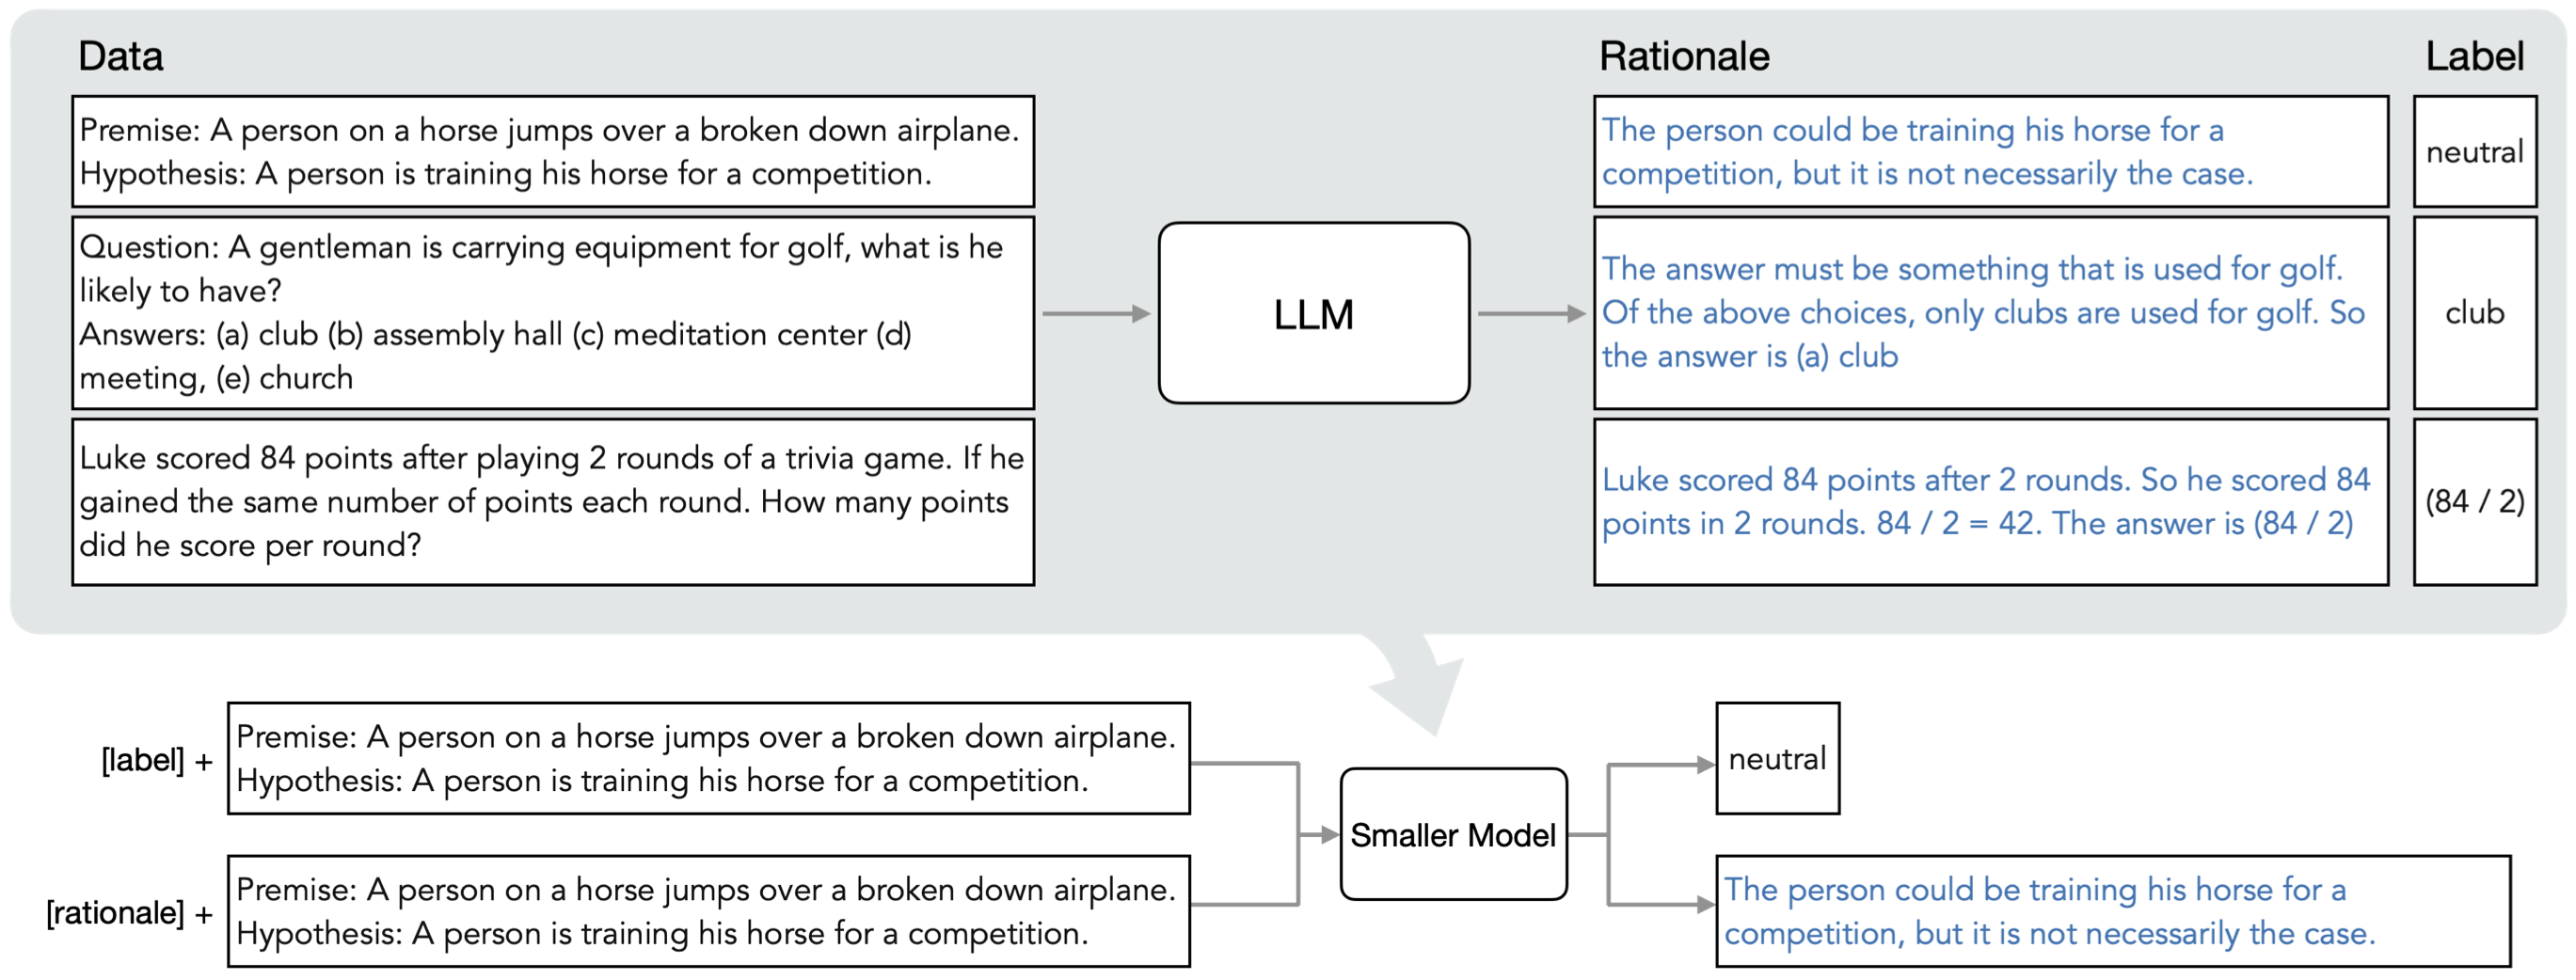
\includegraphics[width=0.99\linewidth]{figs/stepbystep.png}
    \caption{Overview on Distilling step-by-step method. Source: \cite{stepbystep}.}
    \label{fig:stepbystep}
\end{figure}

The TinyLLM method \cite{tinyllm} improves the previous method by acquiring rationales from multiple LLMs. The authors introduce an optional in-context example generator to produce context-specific examples for a given input to ensure that these teacher-generated rationales are contextually grounded. The student model is trained through multi-task instruction tuning \cite{t5,t0}, including the ground truth label.

\section*{Conclusion}

While the literature on model distillation provides comprehensive insights into its application in ML, a noticeable research gap exists in the specific context of Large Language Models. The unique challenges posed by the immense size and complexity of LLM call for distillation techniques that currently need to be explored. Addressing this gap by developing or optimizing distillation methods specifically for LLM could significantly enhance their computational efficiency and broaden their practical applicability, especially in resource-limited scenarios. This area of research promises to advance the field of ML and make the benefits of LLM more accessible and sustainable.

\chapter{Methodology}
\label{chap:met}

The primary objective of this research endeavor is to investigate the process of distilling an LLM into a sequence classification model (hereafter referred to as ``the classifier'') and to evaluate the efficacy of this methodology in comparison with alternative approaches. These alternatives include constructing a classifier from the ground up, fine-tuning a pretrained classifier, and implementing a black-box knowledge distillation technique onto an LLM\@. The efficacy of the models under consideration will be quantitatively assessed based on the accuracy of their predictions on a designated test set.

This chapter details the architecture of the student model and its training process. After that, I provide an elaborate description of the experimental setup, which includes the datasets in use, the architecture of the models under examination, the employed knowledge distillation techniques, and the adopted effectiveness metrics. This systematic exposition aims to furnish a clear understanding of the methodologies employed and facilitate a rigorous analysis of their relative merits and demerits in the context of enhancing model performance and efficiency.

% The distillation methods proposed is inspired by reviewed black-box LLM distillation methods (\autoref{section:blackbox}). Authors demonstrate how to leverage the deep insights of large models to guide the training of compact models using rationale generated by LLM (\autoref{fig:stepbystep}). This rationales offer a more in-depth insight into the reasoning behind associating an input with a particular output label. Provided approach serves as a foundation for developing a more efficient and effective distillation method tailored specifically for sequence classification models.

\section{Datasets}

The datasets selected for this study specifically chosen for their applicability to the research at hand. The primary criterion for dataset selection is their relevance to classification tasks. Through this targeted dataset selection, the research aims to rigorously evaluate the effectiveness of incorporating rationales into the training process of classification models.

\subsection{Extended Stanford Natural Language Inference (e-SNLI)}
\label{sec:esnli}

For the exploration of the student model's capabilities in classification tasks, we specifically focus on Natural Language Inference (NLI) datasets within the scope of this research. NLI datasets are pivotal for evaluating the model's proficiency in understanding and processing human language, offering a rich ground for testing its ability to deduce the logical relationship between premises and hypotheses. These datasets consist of sentence pairs annotated with labels indicating whether the hypothesis is true (entailment), false (contradiction), or undetermined (neutral) based on the premise. This dataset was chosen because it is highly suitable for building zero-shot classification pipelines \cite{zeroshotclf}, where the model must accurately categorize data points into classes it has not explicitly been trained on, guided by the nuanced comprehension and application of language and logic facilitated by the LLM knowledge.

Extended Stanford Natural Language Inference (e-SNLI) \cite{esnli} is an extension of the Stanford Natural Language Inference (SNLI) dataset \cite{snli}, which is a widely used benchmark for evaluating NLI models. To create it annotators were instructed to judge the relation between sentences given that they describe the same event. Each pair is labeled as ``entailment'', ``neutral'', ``contradiction''. This dataset is particularly useful for evaluating the model's ability to generalize to unseen data and to handle complex and nuanced language constructs.

I have used already generated in \cite{stepbystep} rationales. The authors utilize the Chain-of-Thought (CoT) \cite{cot} prompting approach to instruct LLM on generating rationales. This method involves creating a prompt template that contains triplets of example inputs, their corresponding labels, and user-provided rationales explaining the reasoning behind each association. By appending each dataset input to this template and using it to prompt the PaLM 540B LLM \cite{palm}, the authors guide the model to produce both rationales and labels for each input. This process enables the LLM to replicate the demonstrated reasoning in the template, generating coherent rationales that explain the logic leading to its predictions. The example of the collected data is depicted on Fig. \ref{fig:rationale_dataset}.

\begin{figure}[hbt]
    \centering
    \begin{subfigure}[t]{.5\linewidth}
        \centering
        \lstinputlisting[breaklines=true,breakatwhitespace,breakindent=0em,basicstyle=\footnotesize]{figs/data_example_1.txt}
    \end{subfigure}%
    \begin{subfigure}[t]{.5\linewidth}
        \centering
        \lstinputlisting[breaklines=true,breakatwhitespace,breakindent=0em,basicstyle=\footnotesize]{figs/data_example_2.txt}
    \end{subfigure}

    \caption{Data examples from the e-SNLI dataset, refined with rationale.}
    \label{fig:rationale_dataset}
\end{figure}

The dataset initially comprised 569,033 samples, with each sample annotated with an original label, an LLM-predicted label, and an LLM-provided rationale. For specific reasons related to ensuring consistency and reliability in training and evaluation, I excluded samples where the original label did not align with the LLM prediction label. This curation process resulted in a refined dataset consisting of 399,566 samples. Resulting dataset is available at \linebreak \url{https://hf.co/datasets/batalovme/esnli_with_rationale}.

\subsection{Web Of Science (WOS-11967)}
\label{sec:wos}

For classic multi-class classification task, I selected the WOS-11967 dataset \cite{wos}, which comprises 11,967 documents distributed across 35 categories. By focusing solely on these parent categories, the dataset provides an excellent foundation for evaluating the model’s performance in classifying documents into discrete categories. This choice is particularly advantageous because the dataset encompasses a diverse array of topics, presenting a significant challenge to the model's ability to accurately discern and categorize content that is both complex and varied. The distribution of the classes within the dataset is illustrated in \autoref{fig:wos_distrib}.

\begin{figure}[hbt]
    \centering
    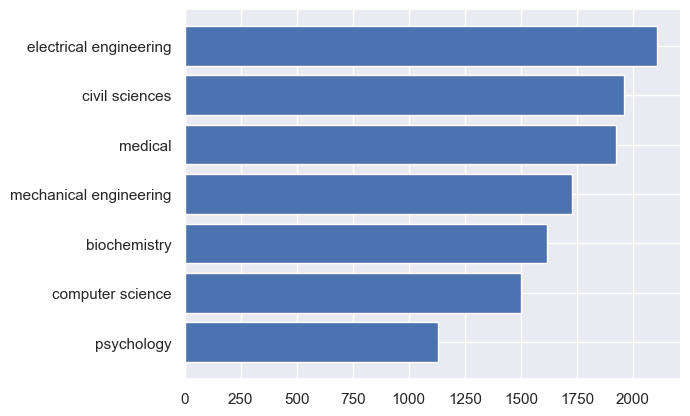
\includegraphics[width=0.8\linewidth]{figs/wos_distrib.png}
    \caption{The class distribution of the sample of the WOS-11967 dataset}
    \label{fig:wos_distrib}
\end{figure}

To conserve resources typically expended on extracting rationales from LLM, I strategically extracted a subset of 4,787 samples from the dataset maintaining the same class distribution as the original. This method not only streamlines the computational demands but also allows for a more focused examination of the model's capability to handle and classify data effectively under conditions of a substantially reduced dataset size.

For the generation of rationales within the dataset, I employed a methodology similar to the one used for the e-SNLI dataset, focusing initially on the creation of two example rationales for each category for few-shot learning with the LLM\@. These rationales were generated by prompting GPT-3.5 using prompt depicted at \autoref{fig:wos_eg_prompt}.

\begin{figure}[ht!]
    \centering
    \lstinputlisting[columns=fullflexible,basicstyle=\small,breaklines=true,breakatwhitespace,breakindent=0em,xleftmargin=1.5cm,xrightmargin=1.5cm,backgroundcolor=\color{lightgray},frame=tlbr,framesep=0.5cm,framerule=0pt]{figs/wos_example_prompt.txt}
    \caption{Prompt for generating example rationales (for few-shot prompting) for the WOS-11967 dataset.}
    \label{fig:wos_eg_prompt}
\end{figure}

After collecting this samples for few-shot learning, I conducted a thorough manual review of each entry. This step was crucial to ensure the quality and consistency of the example shots for the LLM\@.

Using these curated example rationales, I engaged GPT-3.5 in a few-shot learning scenario, where the model was fed with the eamples along prompt to generate rationales.

\begin{figure}[ht!]
    \centering
    \lstinputlisting[columns=fullflexible,basicstyle=\small,breaklines=true,breakatwhitespace,breakindent=0em,xleftmargin=1.5cm,xrightmargin=1.5cm,backgroundcolor=\color{lightgray},frame=tlbr,framesep=0.5cm,framerule=0pt]{figs/wos_prompt.txt}
    \caption{Prompt for generating rationales for the WOS-11967 dataset.}
    \label{fig:wos_prompt}
\end{figure}

This rigorous process ensures that the rationales are not only generated efficiently but are also of high quality and consistent, thereby enhancing the reliability of the dataset for subsequent machine learning tasks.

Resulting dataset consists of 4,787 samples, each annotated with an original label and an LLM-provided rationale. The dataset is available at \linebreak \url{https://hf.co/datasets/batalovme/wos_with_rationale}.

\section{Baseline models and methods}

In the evaluation of sequence classification methodologies, it is imperative to establish robust baseline models for comparison. The baseline models serve as a benchmark against which the efficacy of the distillation process from LLMs to sequence classification models can be measured. This section provides a comprehensive description of the baseline models considered in this study and its results on the datasets under examination.

\subsection{RoBERTa (Robustly Optimized BERT Approach)}

Developed by \citeauthor{roberta} \cite{roberta}, RoBERTa is an enhanced version of BERT (Bidirectional Encoder Representations from Transformers) \cite{bert}, optimized for more robust performance in natural language processing (NLP) tasks.

For sequence classification tasks, RoBERTa utilizes a specialized structure within the Transformer's encoder architecture. Instead of employing a separate decoder, the model leverages the output of a special classification token, commonly known as the CLS token, which is added at the beginning of every input sequence. During pre-training, RoBERTa learns to embed a rich representation of the entire input sequence into this CLS token. This representation is then typically passed through a simple feed-forward network to produce the probability distribution over the possible classes.

\subsection{T5 (Text-to-Text Transfer Transformer)}

Introduced by \citeauthor{t5} \cite{t5}, T5 redefines the approach to NLP tasks by treating every task as a text-to-text problem. This model simplifies the application of transfer learning by using a unified framework across different tasks, including sequence classification.

T5's architecture is based on the Transformer model, which consists of an encoder-decoder structure. The encoder processes the input text, while the decoder generates the output text. In the context of sequence classification, the model is trained to predict the class label based on the input text. This process involves encoding the input text and decoding it to generate the class label as a text.

\subsection{EncT5}

The second variant of the T5 model -- EncT5, which only utilizes the pre-trained encoder part \cite{enct5}. This variant is particularly well-suited for sequence classification tasks, as it focuses solely on the input text and does not require the generation of output text. This model configuration, which avoids the generative complexities of the decoder, utilizes a single `0 token logits' mechanism where a specifically mapped embedding of this token is learned during training to pool information effectively from the entire encoder output. By focusing solely on the encoder and optimizing the information pooling process, EncT5 achieves computational efficiency and simplifies the model architecture.

\subsection{Distilling Step-by-Step!}

Another variant of the T5 model is the methodological framework developed by \citeauthor{stepbystep} \cite{stepbystep}. In their approach, the authors employ LLM rationales as a supplementary source of supervision during the training of smaller, task-specific models within a comprehensive multi-task learning framework. 

The first task is dedicated to generating labels that are direct annotations corresponding to the data instances, facilitating a straightforward supervised learning process. The second task involves the generation of rationales, which are explanatory texts that elucidate the reasoning behind the labels provided by the model. This rationales generation task prefix serve not only to augment the transparency of the model’s decisions but also to provide additional contextual data that aids in refining the training of the seq2seq student models.

At the inference stage, the model employs only the task prefix associated with label generation. This strategic focus ensures that the output is streamlined for practical application, omitting the rationale generation process to enhance efficiency and response time in real-world operational settings. Such an approach underscores the model's adaptability and its potential for application in scenarios where quick decision-making is paramount. Overview on this methodology is illustrated in \autoref{fig:stepbystep}.

\begin{figure}[hbt]
    \centering
    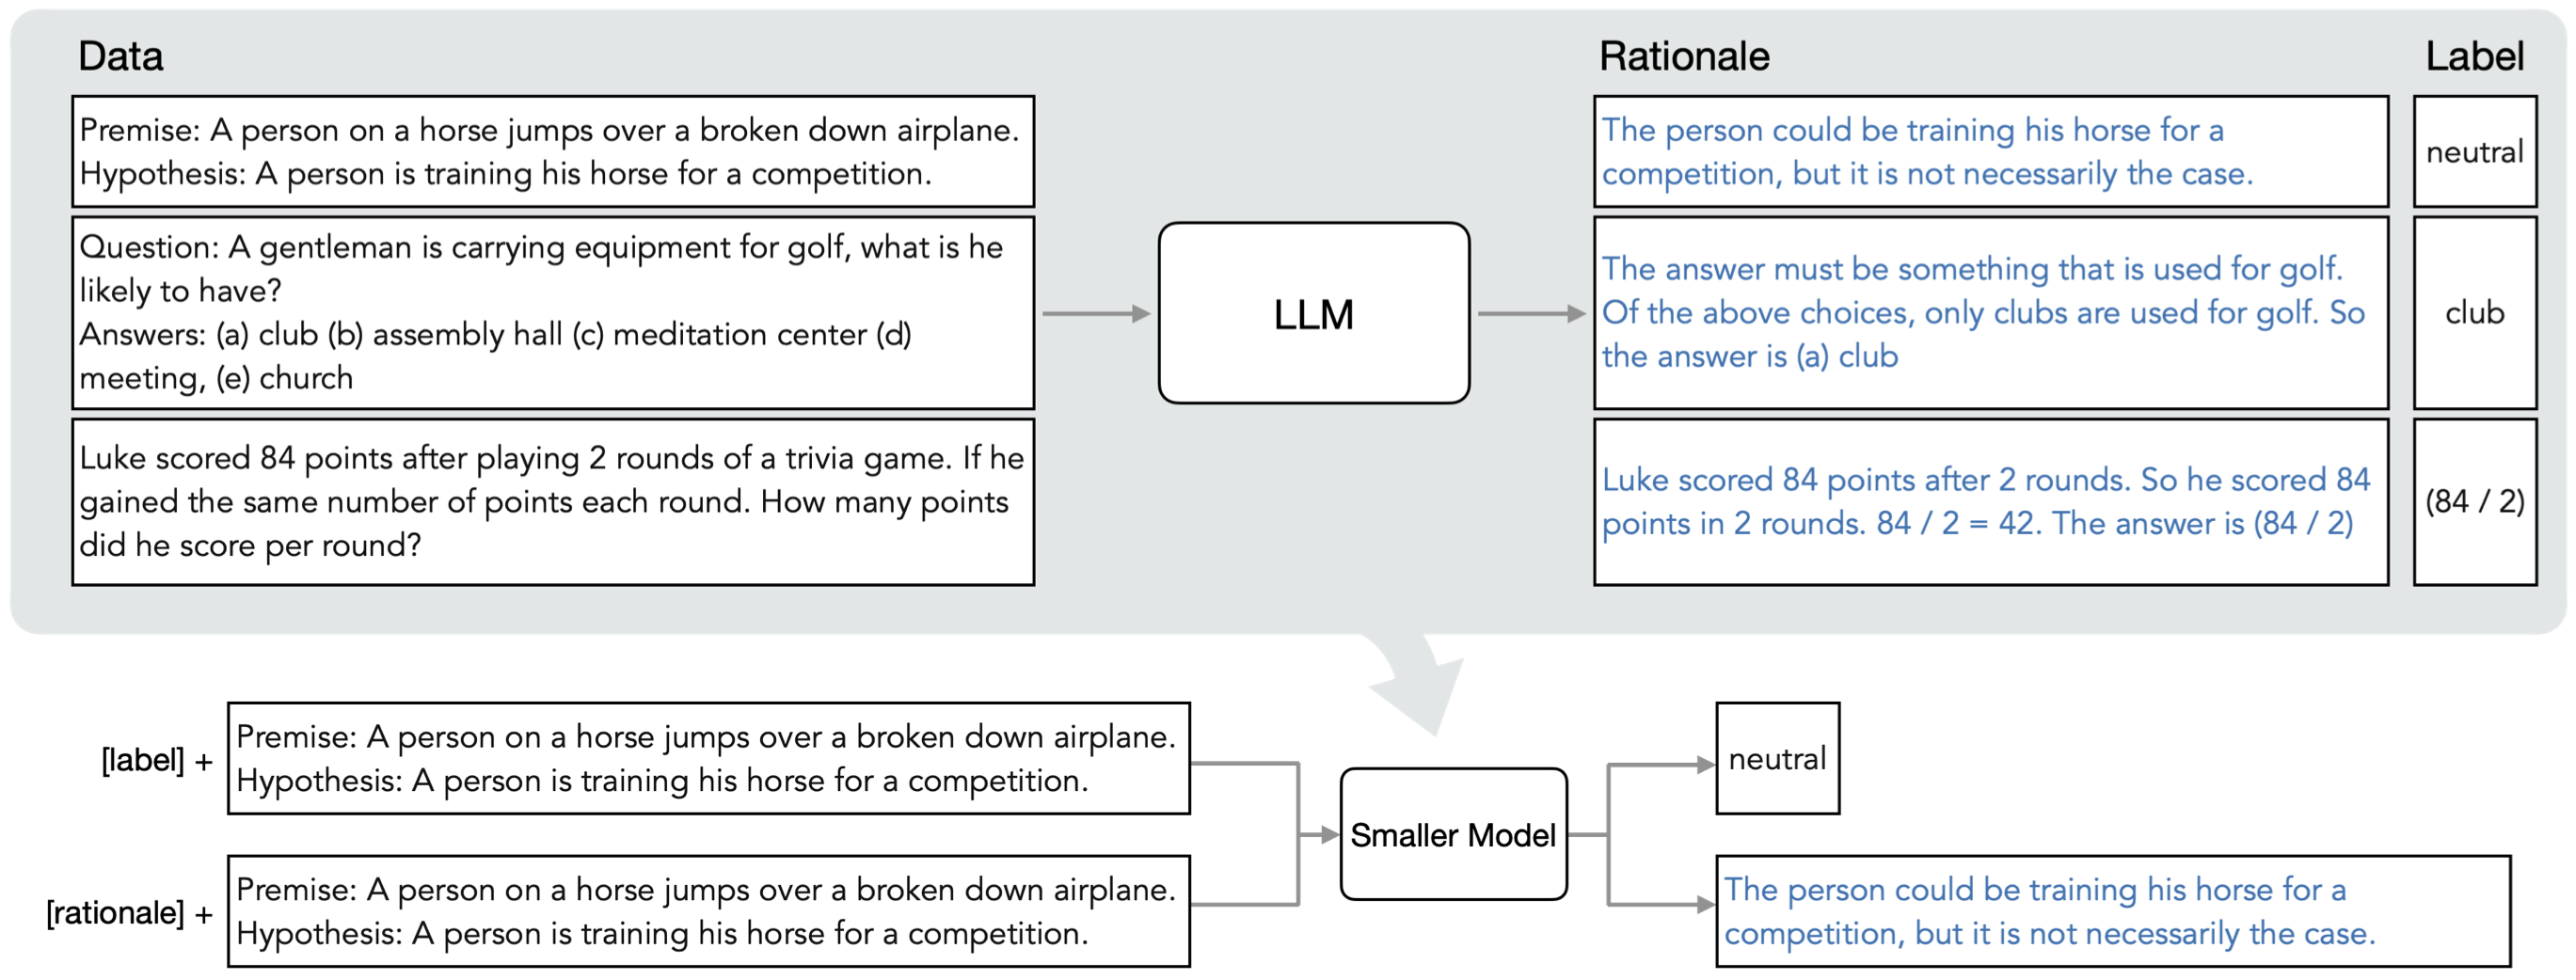
\includegraphics[width=0.99\linewidth]{figs/stepbystep.png}
    \caption[Overview on Distilling step-by-step method.]{Overview on Distilling step-by-step method. Source: \cite{stepbystep}.}
    \label{fig:stepbystep}
\end{figure}

\section{Metrics for evaluation}

The evaluation of classification models on the provided datasets necessitates a comprehensive analysis using standard performance metrics. To accurately gauge the effectiveness of models deployed on these datasets, we employ a suite of metrics: accuracy, precision, recall, and F1 score.

Each metric provides unique insights into different aspects of the model's performance, thus facilitating a robust assessment of its capabilities in handling text classification tasks.

\subsection{Accuracy}

Accuracy is the most commonly used metric for evaluating performance in classification tasks. Accuracy represents the proportion of total predictions that the model classified correctly. It is calculated as the ratio of correctly predicted observations:
$$
    \text{Accuracy} = \frac{\text{Number of Correct Predictions}}{\text{Total Number of Input Data}}
$$

This metric is particularly straightforward and provides an immediate understanding of the overall effectiveness of the model. Fortunately, the same metric used in binary classification can be applied to multi-class classification problems without any modification.

However, it may not always be the most reliable metric in datasets with imbalanced classes. In scenarios characterized by class imbalance, reliance on accuracy as a metric can be deceptive. It often presents an inflated score, despite the model's inadequate performance in predicting minority classes. For instance, consider an evaluation set where there are eight instances of class 0 and two instances of class 1. If a model consistently predicts class 0 for all inputs, it would achieve an accuracy of $80\%$. However, this does not signify a well-performing model, as it completely fails to identify any instances of the minority class.

To gain a more comprehensive understanding of a classifier's performance in situations of class imbalance, it is advisable to examine metrics such as precision and recall. These metrics offer a more nuanced insight into the classifier's error dynamics across different classes, thereby revealing its effectiveness in correctly identifying each class.

\subsection{Understanding True Positives, False Positives, True Negatives, and False Negatives}

To facilitate a deeper understanding of the other metrics discussed, it is imperative to define the core components that constitute these measurements: True Positives (TP), False Positives (FP), True Negatives (TN), and False Negatives (FN). These terms are foundational in constructing the confusion matrix, a tool used to visualize the performance of a binary classification model. Below, I present a \autoref{tab:confusion_matrix} that elucidates these components.

\begin{table}[h]
    \centering
    \caption{Confusion Matrix}
    \begin{tabular}{|c|c|c|}
        \hline
                                          & \multicolumn{2}{c|}{\textbf{Predicted}}                       \\ \cline{2-3}
        \multirow{-2}{*}{\textbf{Actual}} & Positive                                & Negative            \\
        \hline
        Positive                          & True Positive (TP)                      & False Negative (FN) \\
        \hline
        Negative                          & False Positive (FP)                     & True Negative (TN)  \\
        \hline
    \end{tabular}

    \label{tab:confusion_matrix}
\end{table}


\subsection{Precision}

Precision, or positive predictive value, measures the accuracy of the positive predictions made by the model. It is defined as the ratio of true positive predictions to the total predicted positives:

$$
    \text{Precision} = \frac{\text{True Positives}}{\text{True Positives} + \text{False Positives}}
$$

Essentially, precision evaluates the model's ability to correctly identify instances of a specific class. This metric is essential in situations where the consequences of a false positive are significant, such as in document classification tasks within the WOS (\autoref{sec:wos}). High precision is crucial for ensuring documents are accurately categorized, thereby minimizing the risk of misclassification. 

\subsection{Recall}

Recall, also known as sensitivity or true positive rate, quantifies the model's ability to identify all relevant instances within a dataset. It is calculated as follows:

$$
    \text{Recall} = \frac{\text{True Positives}}{\text{True Positives} + \text{False Negatives}}
$$

In simpler terms, recall evaluates the model's capability to detect every instance of a specific class. High recall is crucial in critical applications where missing true positives could lead to dire outcomes. For example, in the e-SNLI dataset (\autoref{sec:esnli}), achieving high recall implies that the model effectively recognizes the majority of accurate entailments, contradictions, or neutral statements based on the provided premises.

The most detailed and intuitive explanation of the metrics precision and recall is provided at the \autoref{fig:precisionrecall}.

\begin{figure}[h!]
    \centering
    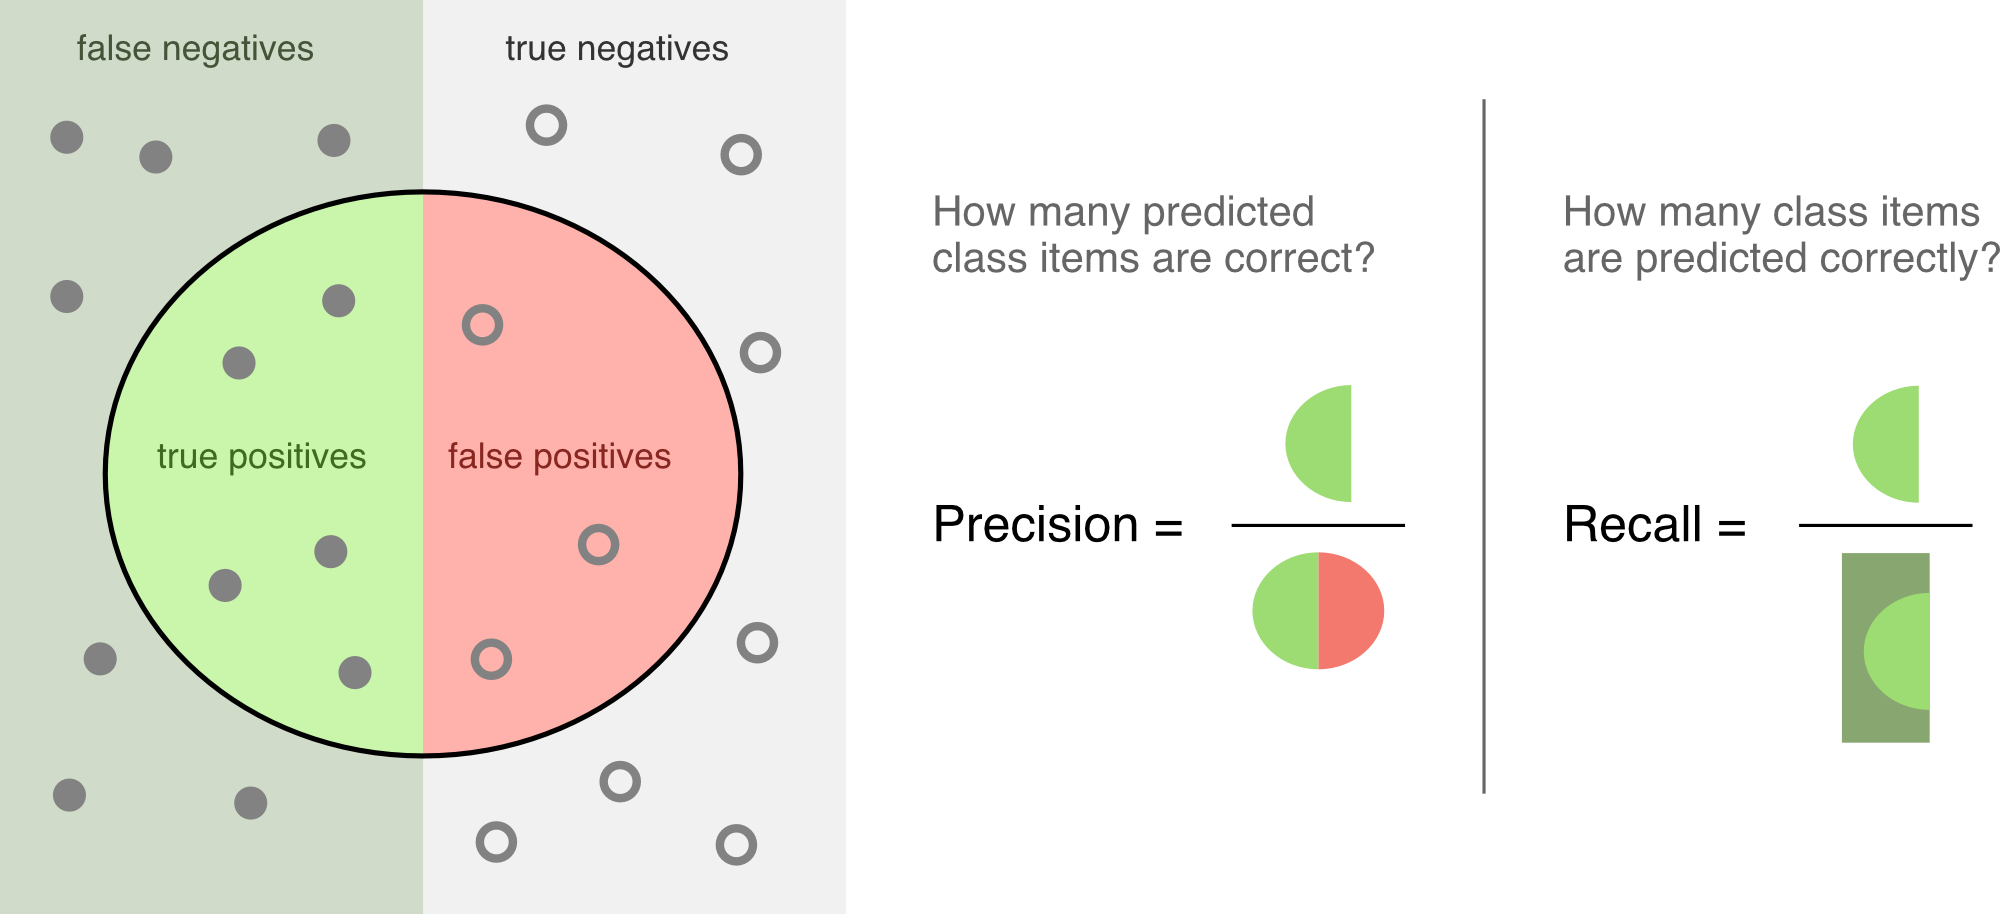
\includegraphics[width=0.9\linewidth]{figs/precisionrecall.jpg}
    \caption[Precision and recall]{Precision and recall. Adopted from Wikipedia\protect\footnotemark.}
    \label{fig:precisionrecall}
\end{figure}


\subsection{F1 Score}
The F1 score is the harmonic mean of precision and recall, providing a balance between the two by taking both false positives and false negatives into account:

$$
    \text{F1 Score} = 2 \times \frac{\text{Precision} \times \text{Recall}}{\text{Precision} + \text{Recall}}
$$

This metric is particularly useful when there is an uneven class distribution, as is common in many real-world datasets, including those in NLP tasks like used in this study. The F1 score serves as a single measure to capture both aspects of model accuracy concerning positive class predictions.

\footnotetext{Source available at \url{https://en.wikipedia.org/wiki/Precision_and_recall}}

\section{Knowlegde distillation methods}
\chapter{Experiments \& Results}
\label{chap:impl}

This chapter presents a comprehensive examination of various experiments designed to investigate the effectiveness of knowledge distillation techniques in enhancing the performance of smaller models through the utilization of LLM\@. 

The experiments are systematically structured to compare baseline models, explore innovative architectural modifications, and assess the impact of training strategies on model accuracy and efficiency in sequence classification tasks. The experimental findings are crucial for validating the theoretical propositions discussed in previous chapters and for demonstrating the practical capabilities of distillation methodologies in real-world applications.

Additionally, this chapter aim to deepen the understanding of knowledge distillation processes and their practical applications in enhancing the efficacy of smaller models by leveraging the knowledge embedded within LLM\@. The results from these experiments will provide valuable insights that could reshape approaches to model training and optimization in the field of NLP\@.

\newcounter{experiment}
\stepcounter{experiment}
\section{Experiment \theexperiment: Evaluating the baselines}

In this section, I detail the methodologies and results of the experiment aimed at evaluating the baseline models described in \autoref{sec:baselines}. The primary goal of this experiment is to assess the performance of each model across datasets provided in \autoref{sec:datasets} to establish a benchmark for future comparative analyses.

Prior to the training process, the datasets were segmented into smaller portions (\autoref{tab:dataset_portions}). The rationale behind selecting varied dataset sizes, including smaller subsets and relatively larger subsets, is to enable a more precise evaluation of model distillation techniques across different scales of data. This approach allows for a detailed comparison of how data volume impacts the effectiveness of distillation in transferring knowledge from larger to smaller models. This standardized approach is crucial for mitigating variability in dataset size, which can influence the accuracy and reliability of the results, particularly when assessing model performance under different data constraints.

\begin{table}[h]
    \centering
    \caption{Number of samples in each dataset portion}
    \label{tab:dataset_portions}
    \resizebox{\textwidth}{!}{
        \begin{tabular}{lccccccccc}
            \toprule
                                         & \multicolumn{9}{c}{\textbf{Portion size}}                                                                                                                            \\
            \textbf{Dataset}             & \textbf{0.01}                             & \textbf{0.03} & \textbf{0.05} & \textbf{0.07} & \textbf{0.1} & \textbf{0.3} & \textbf{0.5} & \textbf{0.7} & \textbf{1.0} \\

            \midrule
            WOS (\autoref{sec:wos})      & N/A                                       & N/A           & N/A           & N/A           & 380          & 1,138        & 1,896        & 2,654        & 3,791        \\
            e-SNLI (\autoref{sec:esnli}) & 386                                       & 1,156         & 1,926         & 2,697         & 3,852        & 11,556       & 19,260       & 26,964       & 38,520       \\
            \bottomrule
        \end{tabular}
    }
\end{table}

Each model was trained on the datasets using a predefined split of training and validation data, same for each model. Model validation was performed intermittently during training to monitor performance, adjust parameters as necessary and use early stopping to prevent overfitting.

After training, each model was evaluated on a separate test set that was not used during the training or validation phases. This approach ensures that the performance metrics reflect the generalizability of each model.

The results of this experiment are presented in the Fig. \ref{fig:baselines:wos} and \ref{fig:baselines:esnli}, where the F1 score is utilized as the primary metric for model evaluation. The F1 score, a harmonized measure that incorporates precision, recall, and accuracy, is particularly effective in providing a balanced assessment of model performance.

\begin{figure}[p]
    \centering
    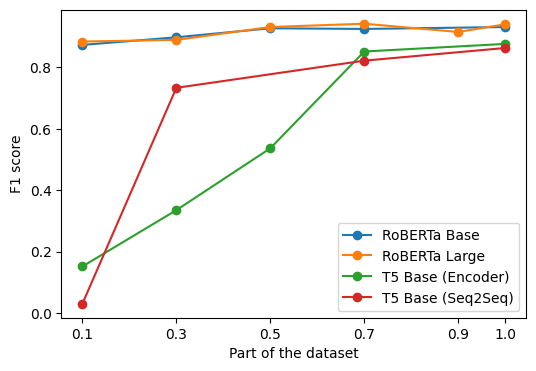
\includegraphics[width=0.6\linewidth]{figs/wos_baseline.png}
    \caption{F1 score performance of baseline models on the WOS dataset across varying dataset sizes.}
    \label{fig:baselines:wos}
\end{figure}
\begin{figure}[p]
    \centering
    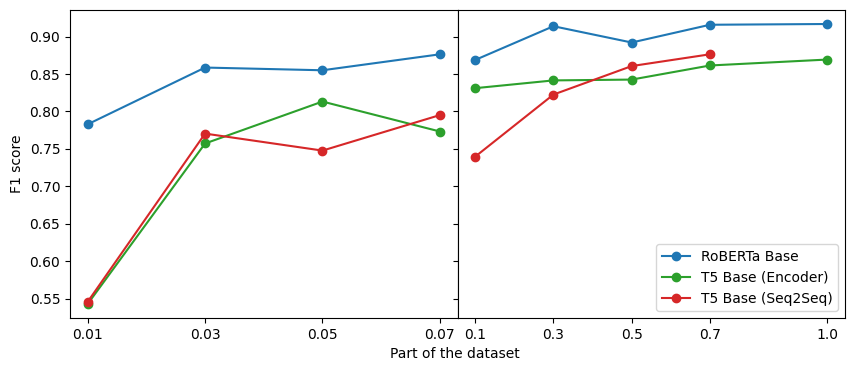
\includegraphics[width=\linewidth]{figs/esnli_baseline.png}
    \caption{F1 score performance of baseline models on the e-SNLI dataset across varying dataset sizes.}
    \label{fig:baselines:esnli}
\end{figure}

These figures vividly illustrate the performance of each model across various dataset sizes, offering a detailed visualization of the models' accuracy and efficiency.

This comprehensive overview allows for a nuanced analysis of how model effectiveness varies with the size of the dataset. RoBERTa models consistently outperformed T5 models, regardless of their setup, across all dataset sizes, demonstrating their superior performance in sequence classification tasks.

Additionally, RoBERTa exhibited less variance across different dataset sizes, indicating more robust and reliable performance. Conversely, the EncT5 model showed little improvement over the T5 Seq2Seq model, suggesting that the architectural modifications did not significantly enhance its classification capabilities.

These insights give rise to the hypothesis that models designed explicitly for classification, like RoBERTa, may be inherently more suitable for student model compared to more generative models like T5.

\newpage

\stepcounter{experiment}
\section{Experiment \theexperiment: Train T5 model with 2 heads}

The student model in this experiment employs a modified T5 architecture \cite{t5}, incorporating a dual-head design to enhance its functionality. This adaptation includes the addition of a classification head alongside the existing language modeling head, which is now specifically tasked with generating rationales (\autoref{fig:modified_t5}). The model is trained on a dataset that consists of labeled examples, with its training trajectory significantly informed by the LLM knowledge. But during the prediction phase, the classification head is used to make predictions, while the language modeling head is not utilized.

\begin{figure}[hbt]
    \centering
    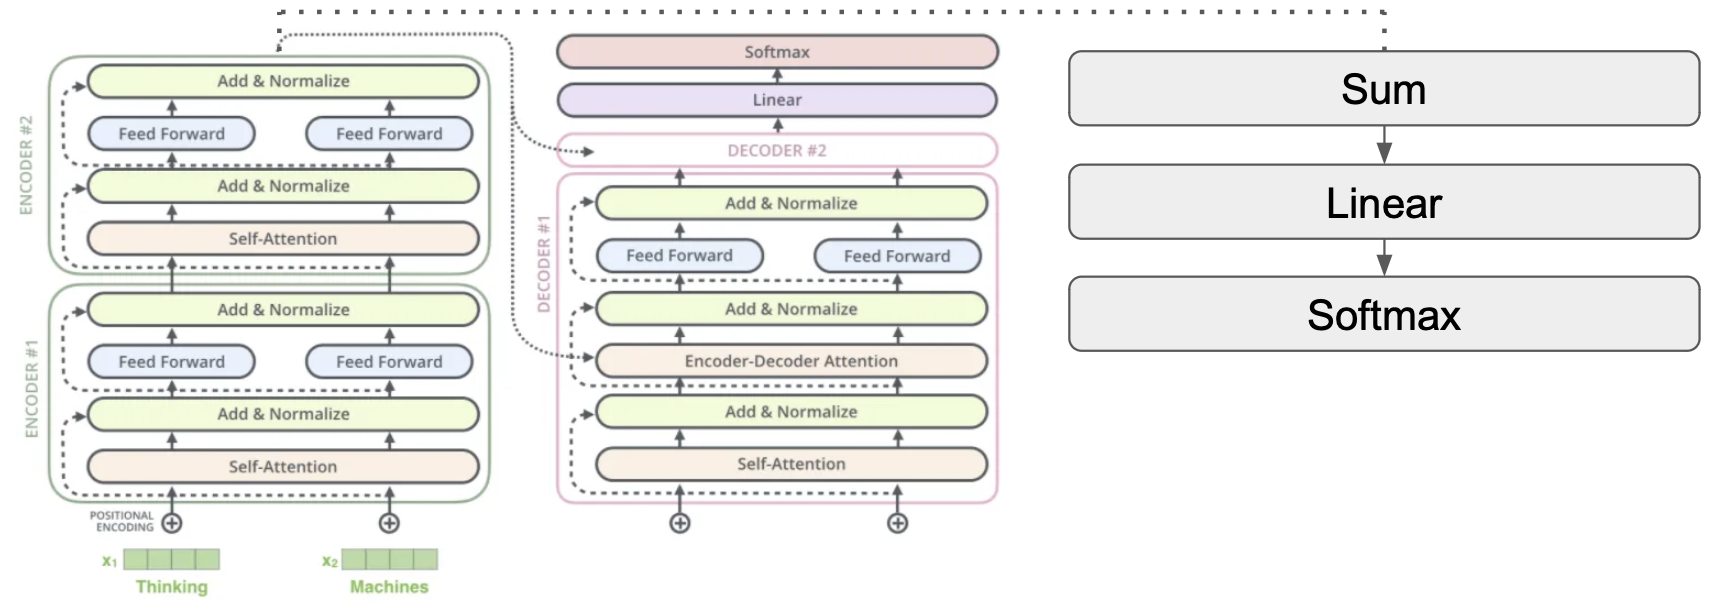
\includegraphics[width=0.99\linewidth]{figs/modified_t5.png}
    \caption{Modified T5 architecture for the student model.}
    \label{fig:modified_t5}
\end{figure}

The use of a linear combination for the loss function optimally balances the contributions from both language modeling and classification tasks during training. Specifically, the combined loss function can be formulated as follows
$$ L = \alpha L_{LM} + (1 - \alpha) L_{C} $$
Where $L$ represents the total loss, $L_{LM}$ is the original T5 language modeling loss, $L_{C}$ is the classification loss (cross-entropy), and $\alpha$ is a hyperparameter that determines the relative importance of the two losses.

Irrespective of the selected value for the parameter $\alpha$, there was no observed reduction in the classification loss. Language modeling loss, exhibited some decrease depends on $\alpha$, indicating that the model was learning to generate rationales. This phenomenon may be attributed to the possibility that the features extracted by the T5 encoder, which are utilized by the decoder, are insufficient for the classification task.

\ldots

\chapter{Analysis and Discussion}
\label{chap:eval}

This chapter delves into the analysis of the experimental results obtained in the previous chapter, focusing on the implications and insights drawn from the performance of various knowledge distillation techniques. The discussion adressed to the central research question ``How black-box distillation effective for sequence classification'' and centers on evaluating the successes and limitations of these methods and considering their theoretical and practical significance within the field of NLP\@.

The experiments conducted have provided valuable data on the utility of knowledge distillation techniques in improving the efficiency and efficacy of smaller models for sequence classification.

The baseline RoBERTa model exhibited superior classification accuracy compared to the T5 model, underscoring its robust performance in sequence classification tasks. This observation indicated that RoBERTa could be a more effective recipient for knowledge distillation, suggesting a promising avenue for enhancing its capabilities through this technique. But, pure rationale-augmented training approach for RoBERTa did not yield the anticipated improvements in performance on test set without rationales. This finding invites a deeper exploration of how context and additional information are integrated into model training processes. 

The T5 model, originally designed for Seq2Seq text generation tasks, demonstrates comparatively lower performance in sequence classification tasks. However, this generative capability positions the T5 model as particularly suitable for generating rationales within a knowledge distillation context. By leveraging its strength in producing detailed and nuanced text, T5 can be effectively utilized to generate explanatory rationales. These rationales can then be used to augment the training data for other models, such as RoBERTa, which excel in classification tasks.

The experimental results also highlighted the importance of generation and integration of rationales into the black-box distillation process. When LLMs like GPT generate rationales, they offer insights into the reasoning behind their outputs. These rationales can be seen as a form of ``unpacking'' the black-box. Depending on the method of deriving rationale from the LLM, the degree of this ``unpacking'' is changed. This distinction is crucial, as it influences the quality and relevance of the rationales generated, which, in turn, affects the performance of the student model.

\section{Results of proposed method on WOS dataset}

The distilation pipeline developed in this research, which combines the generative capabilities of T5 with the classification strengths of RoBERTa, offers a novel approach to enhancing the performance of smaller models. By leveraging the strengths of each model, this pipeline can potentially improve the efficiency and accuracy of sequence classification tasks. The experimental results demonstrated that this pipeline could effectively distill knowledge from the T5 model to the RoBERTa model, resulting in improved performance on the test set of the WOS dataset.

The application of the proposed knowledge distillation method, using rationales generated by the T5 model to train the RoBERTa model, resulted in an increase of 1-2\% in accuracy, precision, recall, and F1 score across experiments on the WOS dataset.

\section{Results of proposed method on e-SNLI dataset}

In contrast, this pipeline did not yield significant improvements in performance on the test set of the e-SNLI\@. This discrepancy suggests that the effectiveness of the distillation pipeline may be influenced by many factors. Further investigation is required to determine the factors that contribute to the success or failure of this distillation process on different datasets.

\section{Limitations and Future Work}

Additionally, the experiments also highlight several limitations in the provided methodology. 

A significant limitation of this study is the exclusion of many potential experimental cases due to constraints in computational resources. The availability of more extensive computational power could have allowed for a broader exploration of model configurations and training setups, possibly uncovering additional insights into the effectiveness of knowledge distillation techniques. This restriction may have resulted in a narrower view of the potential capabilities and optimizations of the models studied.

The results obtained are primarily based on the WOS dataset. While this provides a focused context for observing the impact of the proposed distillation method, it also limits the generalizability of the findings.

The integration of rationales did not significantly enhance model performance for all data. Future work could explore different types of rationale integration or the development of models specifically designed to leverage complex contextual information more effectively.

The scalability of the proposed pipeline under different operational conditions and data volumes remains to be tested. Often, pipelines are more complex in real-world scenarios, and deploying them at scale may introduce additional challenges that were not present in the experimental setup.

By addressing these limitations in future research, there is potential to enhance the robustness of the findings and expand the applicability of knowledge distillation methods in NLP.

\chapter{Conclusion}
\label{chap:conclusion}

\ldots



%% REFERENCES
\printbibliography[heading=bibintoc,title={Bibliography cited}]
\appendix
\renewcommand{\chaptername}{Appendix}
\chapter{Extra Stuff}

\begin{figure}[hbt]
    \centering
    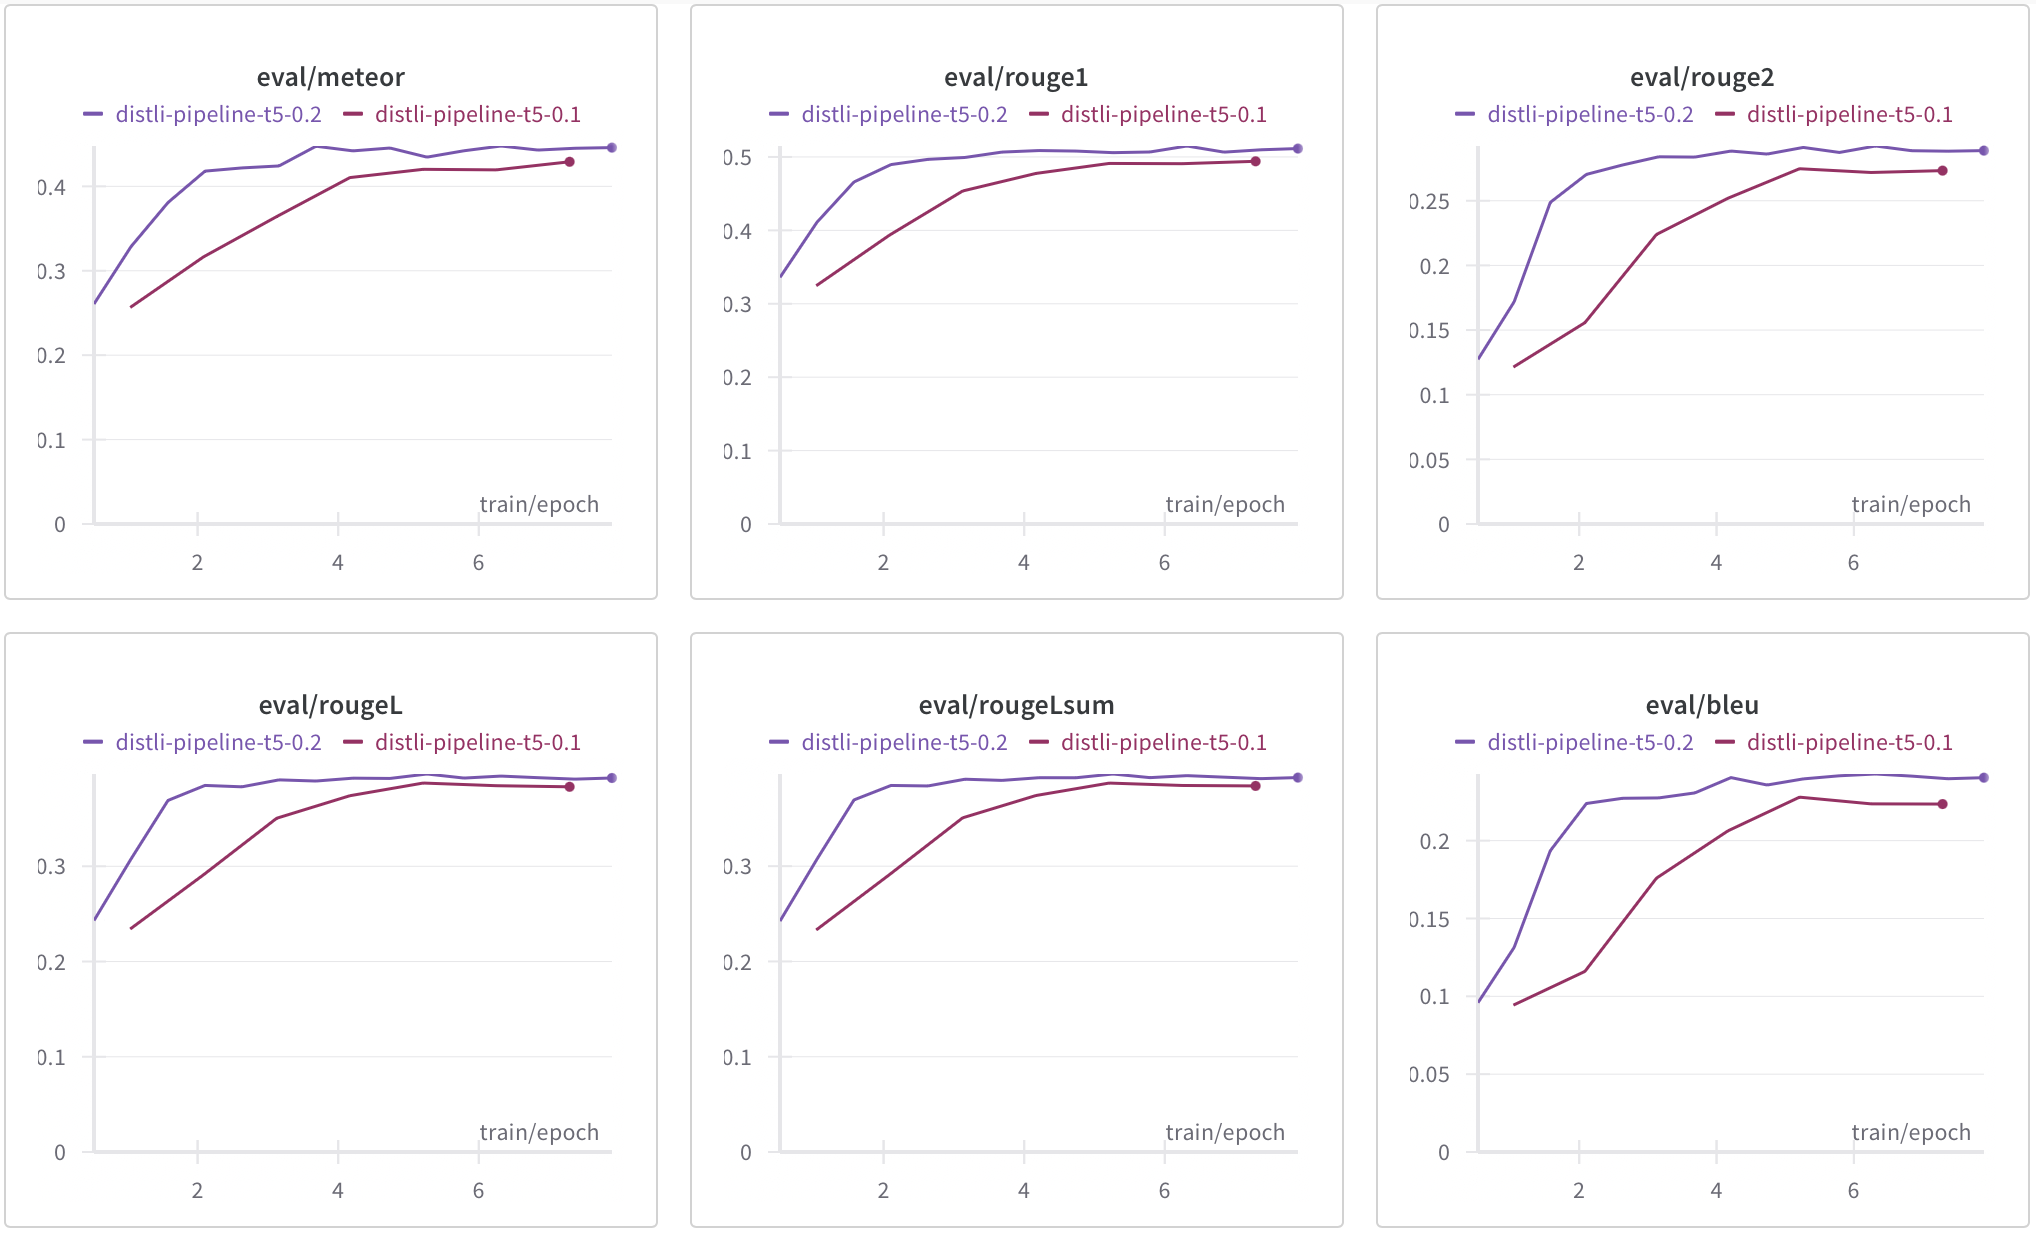
\includegraphics[width=\linewidth]{figs/t5_metrics_wos.png}
    \caption{Evaluation metrics of training T5 model on the rationales of the WOS dataset.}
    \label{fig:t5_metrics_wos}
\end{figure}

\end{document}
